\begin{minipage}{0.75\linewidth}
\begin{figure}[h]
    \centering
    \begin{adjustbox}{max width=1.0\linewidth, keepaspectratio}
        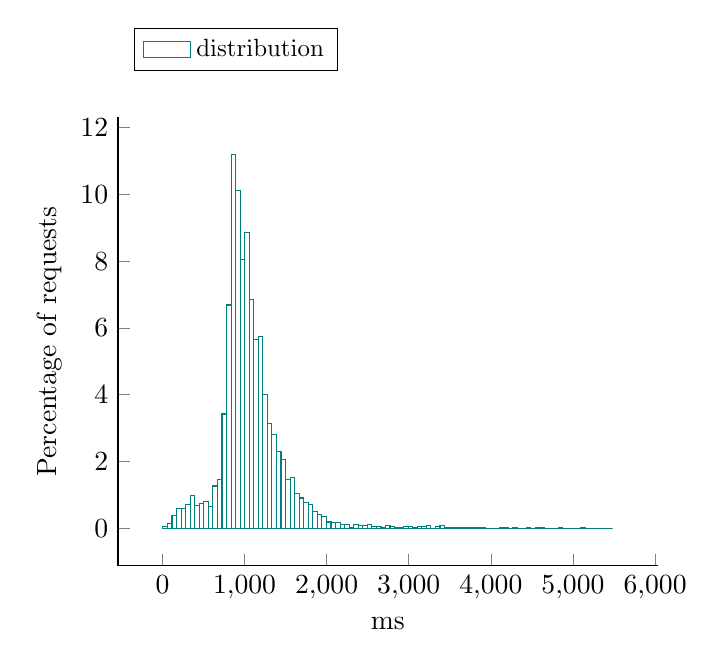
\begin{tikzpicture}
            \begin{axis}[ylabel = Percentage of requests, 
xlabel = ms, 
legend style = {nodes={scale=0.9, transform shape}, at={(0.03,1.2)}, anchor=north west, draw=black, fill=white, align=left, legend columns=3},
area style, mark size = 0pt,
 cycle list name = exotic,
  axis lines* = left]
		\addplot +[ybar interval] coordinates {
			 (6, 0.0625)
			 (61.32, 0.15625)
			 (116.64, 0.390625)
			 (171.96, 0.59375)
			 (227.28, 0.59375)
			 (282.6, 0.703125)
			 (337.92, 0.96875)
			 (393.24, 0.6875)
			 (448.56, 0.75)
			 (503.88, 0.8125)
			 (559.2, 0.640625)
			 (614.52, 1.26562)
			 (669.84, 1.45312)
			 (725.16, 3.42188)
			 (780.48, 6.6875)
			 (835.8, 11.1875)
			 (891.12, 10.1094)
			 (946.44, 8.04688)
			 (1001.76, 8.85938)
			 (1057.08, 6.85937)
			 (1112.4, 5.64062)
			 (1167.72, 5.73438)
			 (1223.04, 4.01562)
			 (1278.36, 3.125)
			 (1333.68, 2.79688)
			 (1389, 2.3125)
			 (1444.32, 2.0625)
			 (1499.64, 1.46875)
			 (1554.96, 1.51562)
			 (1610.28, 1.04688)
			 (1665.6, 0.90625)
			 (1720.92, 0.765625)
			 (1776.24, 0.71875)
			 (1831.56, 0.515625)
			 (1886.88, 0.40625)
			 (1942.2, 0.359375)
			 (1997.52, 0.1875)
			 (2052.84, 0.171875)
			 (2108.16, 0.171875)
			 (2163.48, 0.109375)
			 (2218.8, 0.125)
			 (2274.12, 0.03125)
			 (2329.44, 0.109375)
			 (2384.76, 0.09375)
			 (2440.08, 0.078125)
			 (2495.4, 0.109375)
			 (2550.72, 0.046875)
			 (2606.04, 0.0625)
			 (2661.36, 0.03125)
			 (2716.68, 0.078125)
			 (2772, 0.0625)
			 (2827.32, 0.03125)
			 (2882.64, 0.03125)
			 (2937.96, 0.0625)
			 (2993.28, 0.046875)
			 (3048.6, 0.015625)
			 (3103.92, 0.0625)
			 (3159.24, 0.046875)
			 (3214.56, 0.078125)
			 (3269.88, 0)
			 (3325.2, 0.0625)
			 (3380.52, 0.078125)
			 (3435.84, 0.03125)
			 (3491.16, 0.015625)
			 (3546.48, 0.03125)
			 (3601.8, 0.015625)
			 (3657.12, 0.015625)
			 (3712.44, 0.015625)
			 (3767.76, 0.015625)
			 (3823.08, 0.015625)
			 (3878.4, 0.03125)
			 (3933.72, 0)
			 (3989.04, 0)
			 (4044.36, 0)
			 (4099.68, 0.015625)
			 (4155, 0.015625)
			 (4210.32, 0)
			 (4265.64, 0.03125)
			 (4320.96, 0)
			 (4376.28, 0)
			 (4431.6, 0.015625)
			 (4486.92, 0)
			 (4542.24, 0.015625)
			 (4597.56, 0.03125)
			 (4652.88, 0)
			 (4708.2, 0)
			 (4763.52, 0)
			 (4818.84, 0.03125)
			 (4874.16, 0)
			 (4929.48, 0)
			 (4984.8, 0)
			 (5040.12, 0)
			 (5095.44, 0.015625)
			 (5150.76, 0)
			 (5206.08, 0)
			 (5261.4, 0)
			 (5316.72, 0)
			 (5372.04, 0)
			 (5427.36, 0)
			 (5482.68, 0)
		};
\addlegendentry{distribution};
           \end{axis}
      \end{tikzpicture}
  \end{adjustbox}
  \caption{Response time distribution - req = ReadTimeline-2}
\end{figure}
\end{minipage}\hfill\begin{minipage}{0.18\linewidth}
\begin{table}[h]
\begin{tabular}{|cc|}
\hline
\textbf{} & \textbf{ms}\\ \hline
 \Xhline{0.005\arrayrulewidth}
min & 6\\
 \Xhline{0.005\arrayrulewidth}
max & 5538\\
 \Xhline{0.005\arrayrulewidth}
mean & 1076\\
 \Xhline{0.005\arrayrulewidth}
std & 422\\
\hline
\hline
 \Xhline{0.005\arrayrulewidth}
25th & 868\\
 \Xhline{0.005\arrayrulewidth}
50th & 1012\\
 \Xhline{0.005\arrayrulewidth}
75th & 1216\\
 \Xhline{0.005\arrayrulewidth}
80th & 1285\\
 \Xhline{0.005\arrayrulewidth}
85th & 1378\\
 \Xhline{0.005\arrayrulewidth}
90th & 1501\\
 \Xhline{0.005\arrayrulewidth}
95th & 1728\\
 \Xhline{0.005\arrayrulewidth}
99th & 2748\\
\hline
\end{tabular}
\caption{Response time}
\end{table}
\end{minipage}\hfill